%!TEX program = xelatex
\documentclass[UTF8,a4paper,12pt,twoside]{article}%A4纸,正文为小四号字,对应12pt
%\usepackage{appendix}
\usepackage{tabularx,longtable,threeparttable,booktabs}%表格
\usepackage{diagbox}
\usepackage{multido}
%\usepackage{underscore}
\usepackage{float}
\usepackage{algorithmic}
%\renewcommand{\algorithmname}{算法}
%Add by Karl_Lok
\usepackage[BoldFont,SlantFont,CJKchecksingle]{xeCJK}
\setmainfont{Times New Roman}
\setmonofont{Times New Roman}
\setCJKmainfont{SimSun}
\setCJKmonofont{SimSun}% 设置缺省中文字体
\setCJKfamilyfont{hei}{SimHei} %黑体  hei
% Mac 字体名称与 Windows 不同,需要将宋体和黑体替换为下述注释中内容
% \setCJKmainfont{Songti SC Light}
% \setCJKmonofont{Songti SC Light}
% \setCJKfamilyfont{hei}{Heiti SC Light} %黑体  hei
\newcommand{\hei}{\CJKfamily{hei}}
\setlength{\tabcolsep}{3pt}
\usepackage[hang]{caption2}
\renewcommand{\captionlabeldelim}{\, }   % 改插图题目的冒号为空格
\renewcommand{\captionfont}{\small\hei}
\usepackage{ulem}%下划线,删除线等
\usepackage{xcolor}
\usepackage{listings}
\lstset{escapechar=`,numbers=left
,extendedchars=false, escapeinside=`'
,basicstyle=\ttfamily
,backgroundcolor=\color[RGB]{245,245,244}
,keywordstyle=\bfseries\color[RGB]{130,0,0},identifierstyle=\bfseries\color[RGB]{0,0,130},numberstyle=\color[RGB]{41,41,255},commentstyle=\it\color[RGB]{130,130,130},stringstyle=\rmfamily\slshape\color[RGB]{255,0,0},showstringspaces=false,tabsize=4,texcl=true,frame=shadowbox,breaklines=true,float}
\renewcommand{\lstlistingname}{脚本}
\renewcommand{\lstlistlistingname}{脚本目录}
\usepackage{Style/gzhuThesis}%
\newcommand{\upcite}[1]{$^{\mbox{\scriptsize \cite{#1}}}$} %设置引用,package{cite}

\begin{document}
%!TEX program = XeLaTeX
%!TeX root =main.tex
\classification{}%分类号
\UDC{11078}%学校代码
\studentnumber{xxxxxxxxxx}%学号
\confidential{}%密级
\condate{}%保密日期
\conterm{}%保密期限

\cdegree{硕士学位} %学位
\edegree{Master of Natural Science} %学位英文名
\title{论文中文标题}%在{ }里输入论文题目
\etitle{English Title}%英文题目
\school{物理与电子工程学院}%学院
\eschool{Center for Astrophysics}%学院英文名
\major{天文学}%专业
\emajor{Astronomy}%专业英文名
\field{脉冲星}%方向
\class{xxxx级}%班级
\author{小张}%作者姓名
\eauthor{Y. R. Zhang}%作者英文名
\defcdate{\ctoday}%答辩日期
\defedate{May 2019}%英文格式答辩日期
\supervisor{}%导师姓名及职称
\esupervisor{Prof. H. G. Wang}%导师姓名及职称英文



\begin{titlepage}
\setcounter{page}{0}
\addcontentsline{toc}{section}{封\hspace{1em}面}
%\newgeometry{left=-0.0cm,right=-0.0cm,top=-0.0cm,bottom=-0.0cm}
\newgeometry{left=-0.0cm,right=-0.5cm,top=-0.0cm,bottom=-0.0cm}

\includegraphics[scale=1.0]{logo/HardCover.pdf}\\ %中文A4封面
%\addcontentsline{toc}{section}{声\hspace{1em}明}
%\newpage

\includegraphics[scale=1.0]{logo/Copyright.pdf}\\ %A4版权声明
%\addcontentsline{toc}{section}{扉\hspace{1em}页}
\centerline{
\includegraphics[scale=1.0]{logo/Signature.pdf}} %A4中文扉页
\end{titlepage}
\newpage
 %最后定稿时用来添加封面图片,签名后的版权声明,以及签名后的扉页图片
\makecover %论文中文扉页 最后需注释掉,改用cover.tex中的
\cleardoublepage %
\makeecover  %论文英文扉页
\cleardoublepage
\makeatletter
\makeatother
\newpage
%版权声明,仅为保持论文的完整性,最后会将其注释掉,改用cover.tex中的
%Authorization%%%%%%%%%%%%%%%%%%%%%%%%%%%%%%%%%%%%%%%%%%%%%%%%%%%
    \newpage
   \thispagestyle{empty}
   %\fancyfoot{} % clear all footer fields
    \begin{center}
    {\LARGE \bf{广州大学学位论文原创性声明和使用授权说明}}
   \vspace{0.5cm}
    \parbox[t][1cm][c]{\textwidth}{ {\bf \Large \centerline
    {原创性声明} } }
    \parbox[t][3cm][c]{\textwidth}{ {\fontsize{12pt}{18pt}\selectfont
    \hspace{2em}本人郑重声明:所呈交的学位论文,是本人在导师指导下,独立
    进行研究工作所取得的研究成果。除文中已经标明引用的内容外,本论文不包含
    任何其他个人或集体已经发表或撰写过的研究成果。对本文的研究做出贡献的个
    人和集体,均已在文中以明确方式标明。本声明的法律结果由本人承担。}}
    \parbox[t][2cm][c]{\textwidth}{\fontsize{12pt}{15pt}\selectfont
    \hspace{2em}%\fs
    学位论文作者签名:
    \hspace*{3.3cm} 日期:\hspace{2em}年\hspace{2em}月\hspace{2em}日
    }

    \parbox[t][2cm][c]{\textwidth}{ {\Large \bf \centerline
    {学位论文版权使用授权书} } }
    \parbox[t][3cm][c]{\textwidth}{ {\fontsize{12pt}{18pt}\selectfont
    \hspace{2em}本学位论文作者完全了解学校有关保留、使用学位论文的规定,即:
    学校有权保留并向国家有关部门或机构送交论文的复印件和电子版,允许论文被查阅
    和借阅。本人授权广州大学可以将本学位论文的全部或部分内容编入有关数据库
    进行检索,可以采用影印、缩印或扫描等复制手段保存和汇编本学位论文。}}
   \parbox[t][1.7cm][c]{\textwidth}{\fontsize{12pt}{15pt}\selectfont
   \hspace{2em}%\fs
   学位论文作者签名:
   \hspace*{3.5cm}
   指导教师签名:}
   \parbox[t][1.8cm][c]{\textwidth}{\fontsize{12pt}{15pt}\selectfont
   \hspace{2em} 日期:\hspace{2em}年\hspace{2em}月\hspace{2em}日 %\fs
    \hspace*{2.3cm}日期:\hspace{2em}年\hspace{2em}月\hspace{2em}日
  \vspace{1.5cm}
}
 .\dotfill.
    \parbox[t][2cm][c]{\textwidth}{ {\fontsize{12pt}{18pt}\selectfont
    \hspace{2em}本人已经认真阅读“CALIS高校学位论文全文数据库发布章程”,
    同意将本人的学位论文提交“CALIS高校学位论文全文数据库”中全文发布,
    并可按“章程”中的规定享受相关权益。同意论文提交后滞后:□半年;□一年;□二年发布。}}
   \parbox[t][1.5cm][c]{\textwidth}{\fontsize{12pt}{15pt}\selectfont
   \hspace{2em}%\fs
   学位论文作者签名:
   \hspace*{3.5cm}
   指导教师签名:}
   \parbox[t][0.4cm][c]{\textwidth}{\fontsize{12pt}{15pt}\selectfont
   \hspace{2em} 日期:\hspace{2em}年\hspace{2em}月\hspace{2em}日%\fs
    \hspace*{2.3cm}日期:\hspace{2em}年\hspace{2em}月\hspace{2em}日
    }
    \end{center}
 
\newpage
\cleardoublepage
%正文
\setcounter{page}{1}
\pagenumbering{Roman}
\section*{摘\hspace{1em}要}
\addcontentsline{toc}{section}{摘\hspace{1em}要}
%!TEX program = XeLaTeX
%!TeX root =main.tex
%请在下面输入中文摘要。
中文摘要。
\\
{\flushleft\textbf{\large 关键词}\hspace{2em}}
%!TEX program = XeLaTeX
%!TeX root =main.tex
%请在下面输入中文关键词,以逗号分隔。
脉冲星;模式变换;星表;分类
\\
\newpage
\cleardoublepage
\section*{ABSTRACT}
\addcontentsline{toc}{section}{ABSTRACT}
%!TEX program = XeLaTeX
%!TeX root =main.tex
%请在下面输入英文摘要。
Abstract in English
\\
{\flushleft\textbf{\large KEY WORDS}\hspace{2em}}
%!TEX program = XeLaTeX
%!TeX root =main.tex
%请在下面输入英文关键词,以逗号分隔。
Pulsars;Mode Changing;Catalogue;Classification

\cleardoublepage
\newpage
\tableofcontents%生成目录
\cleardoublepage
\newpage
\setcounter{page}{1}
\pagenumbering{arabic}

%请在下面输入前言内容。
\section{前\hspace{1em}言}
论文第 \ref{sec:Ref}章介绍了两种论文中常见的引用方式,并在第\ref{sec:summ}章做了总结。
 %
\newpage
%!TEX program = XeLaTeX
%!TeX root =main.tex
%请在下面输入本章内容。
\section{文献的引用} \label{sec:Ref}
论文文本中需要引用参考文献来注明出处。

\subsection{在文本中的引用方式} \label{ssec:Txtref} %
引用可分为作为文章内容的普通引用,和只作为注解用的上标引用。

\subsubsection{普通引用} \label{sssec:Tcite} %
引用方式\cite{Designated}为普通引用。

\subsubsection{上标引用} \label{sssec:Tupcite}
有时候还需要用到上标引用\upcite{jiyulisanduishu,cyu282}。

\subsection{在图表中的引用方式} \label{ssec:PnTref}
图表中亦可引用文献,方法与文本中引用相同(见$\S$ \ref{ssec:Txtref})。

\begin{figure}[!ht]
  \centering
  % Requires \usepackage{graphicx}
  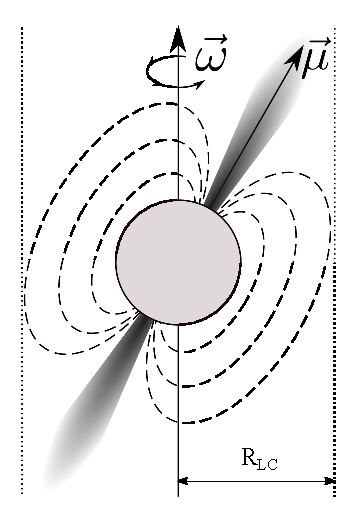
\includegraphics[width=.3\textwidth]{img/lighthouse.eps}\\
  \caption{此处可以引用文献 \upcite{yang_nulling_2014}。}\label{fig:Lighthouse}%{Cooling curve of Pulsars}
\end{figure}


\subsection{小结}
以上为本模板的文献引用方式。
%
\newpage
%!TEX program = XeLaTeX
%!TeX root =main.tex
%请在下面输入本章内容。
\section{总结} \label{sec:summ}
本文绍了两种论文中常见的引用方式。%
\newpage

\addcontentsline{toc}{section}{参考文献}
%\nocite{*}%乱码会报错
\bibliography{paper} %参考文献收录在paper.bib文件
\newpage
\appendix
\titlecontents{section}[0pt]{\vspace{.5\baselineskip}\bfseries}
{\thecontentslabel\quad}{}%附录 %%目录定制
{\hspace{.5em}\titlerule*[10pt]{$\cdot$}\contentspage}
\titleformat{\section}{\centering\xiaoerhao\bfseries}{附录\,\thesection}{1em}{}
\section{论文所用主要代码}\label{sec:code}
\subsection{批量下载图片bash脚本}\label{ssec:download_shell}
\begin{lstlisting}[caption=批量下载图片bash脚本,language=bash]
#!/bin/bash
MAX=\$2;
for ((MAX;MAX>0; MAX--));
        do wget -vv  --no-check-certificate "$1" -O "$MAX";
done;
\end{lstlisting}

\subsection{简单平均法灰度化图片}\label{ssec:gray_pic}
\begin{lstlisting}[caption=简单平均法灰度化图片,language=matlab]
pic=imread('../abc/1');
[h,w,d]=size(pic);
for m=1:h
    for n=1:w
        sum=0;
        for v=pic(m,n,:)
            sum=sum+v/3;
        end
        pic2(m,n)=sum;
    end
end
figure,imshow(pic),figure,imshow(pic2);
\end{lstlisting}


\newpage
\fancyhead[RO,LE]{后\hspace{1em}记}
\section*{后\hspace{1em}记}\addcontentsline{toc}{section}{后\hspace{1em}记}
%!TEX program = XeLaTeX
%!TeX root =main.tex
%此文档为致谢,请在下面直接输入内容。

文本是一个简单的学位论文LaTex模板,可以用作广州大学的本硕博学位论文。

本模板基于广州大学物理与电子工程学院谢老师的本科学位论文模板\footnote{\url{https://github.com/whitelok/GZHU_Latex_Template}} 并参考了考国科大\footnote{\url{https://github.com/mohuangrui/ucasthesis/}}和华中师大学位论文模板,参考文献格式文件基于gbt7714宏包\footnote{\url{https://github.com/CTeX-org/gbt7714-bibtex-style}},默认为GBT7714-2015版,在此对以上作者深表感谢!

强烈建议全国各高校能统一论文格式,大家\footnote{\url{https://github.com/yernhi/collection-latex-templates}}都使用和维护同一个论文模板多方便!

%%% Local Variables:
%%% mode: latex
%%% TeX-master: "main.tex"
%%% End:



\end{document}
